% Chapter Template

\chapter{Diseño e Implementación TECSCI} % Main chapter title

\label{Chapter3} % Change X to a consecutive number; for referencing this chapter elsewhere, use \ref{ChapterX}

%----------------------------------------------------------------------------------------
%	SECTION 1
%----------------------------------------------------------------------------------------
\section{Hardware}

Como se detallo en el capítulo \ref{Chapter2} las primeras pruebas fueron realizadas con la placa experimental TMC5130-EVAL, en la web de la empresa \citep{3_web_trinamic} se pueden encontrar los diseños de todas las placas de evaluación que la misma comercializa. También se analizaron varios esquemáticos de los módulos de desarrollo \textbf{NODE-MCU} del microcontrolador ESP32, este último al ser un producto de venta masiva cuanta con gran cantidad de información y ejemplos de implementaciones. Por lo tanto el diseño de nuestra placa surge del análisis de las implementaciones anteriores.
\\
Para el diseño del \textit{hardware} utilizamos el software libre de diseño de circuitos impresos \textbf{KICAD}, cabe destacar que este software a avanzado y mejorado en cuanto a sus capacidades técnicas en los últimos años, es posible que el apoyo del \textbf{CERN} haya influenciado de manera positiva tal como se comenta en la siguiente nota \citep{1_nota_web_kicad_cern}.

\ref{fig:dip_3d_model}
\ref{fig:dip_real_model}

\begin{figure}[htbp]
	\centering
	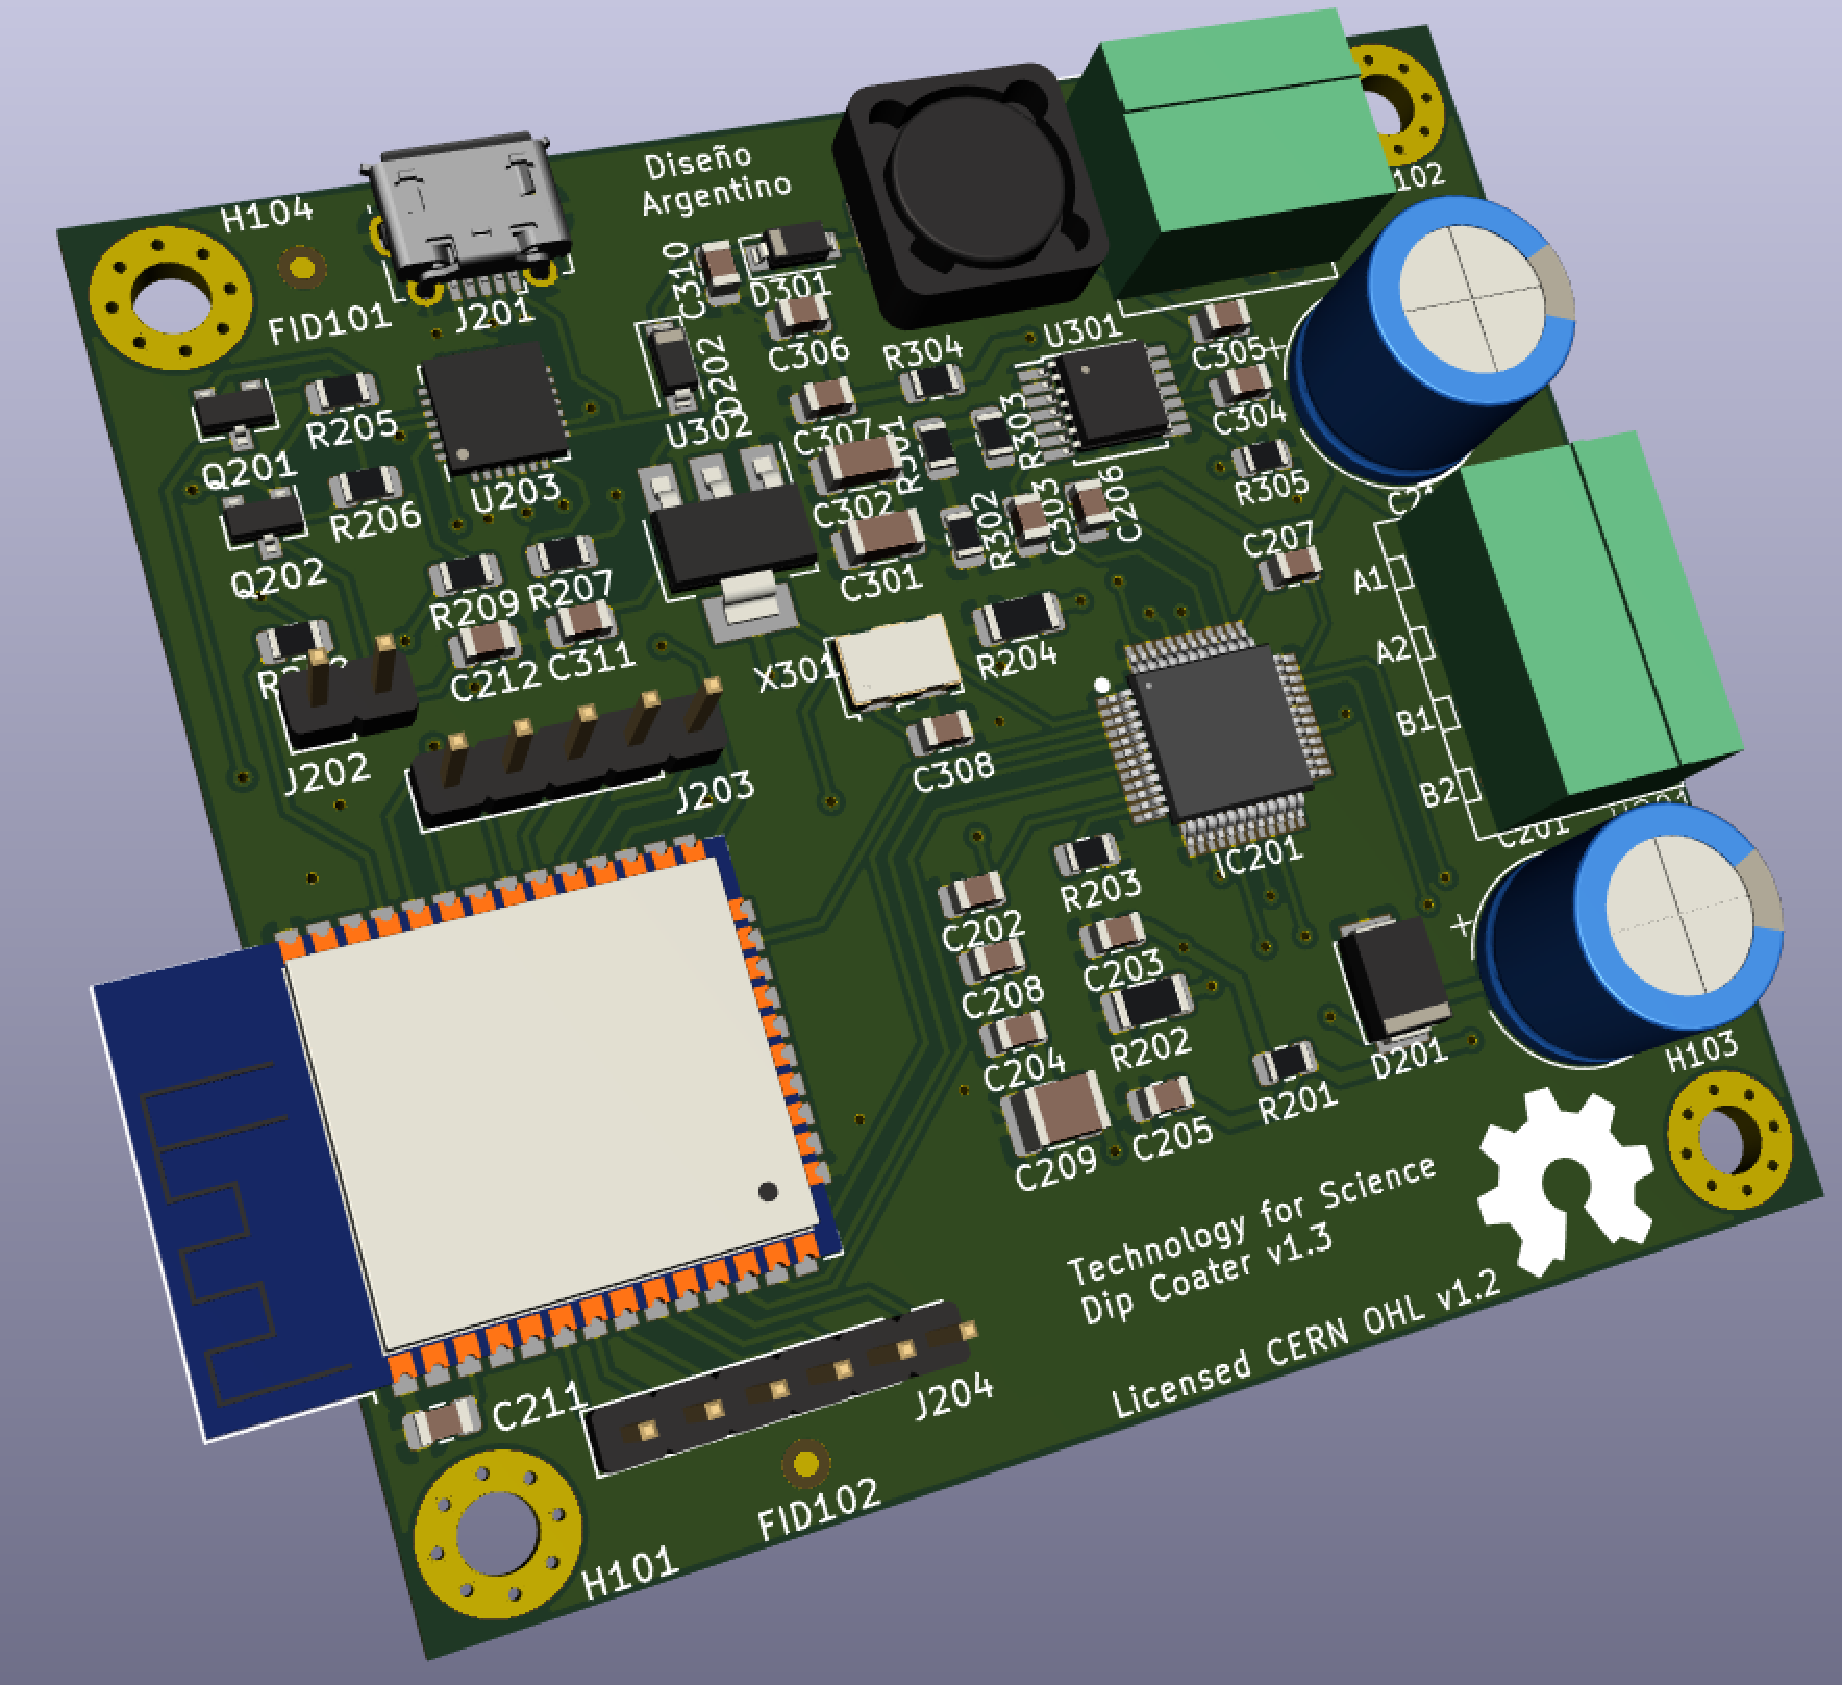
\includegraphics[width=.5\textwidth]{./Figures/dip_3d_model.pdf}
	\caption{Modelo 3D Kicad.}
	\label{fig:dip_3d_model}
\end{figure}
         

\begin{figure}[htbp]
	\centering
	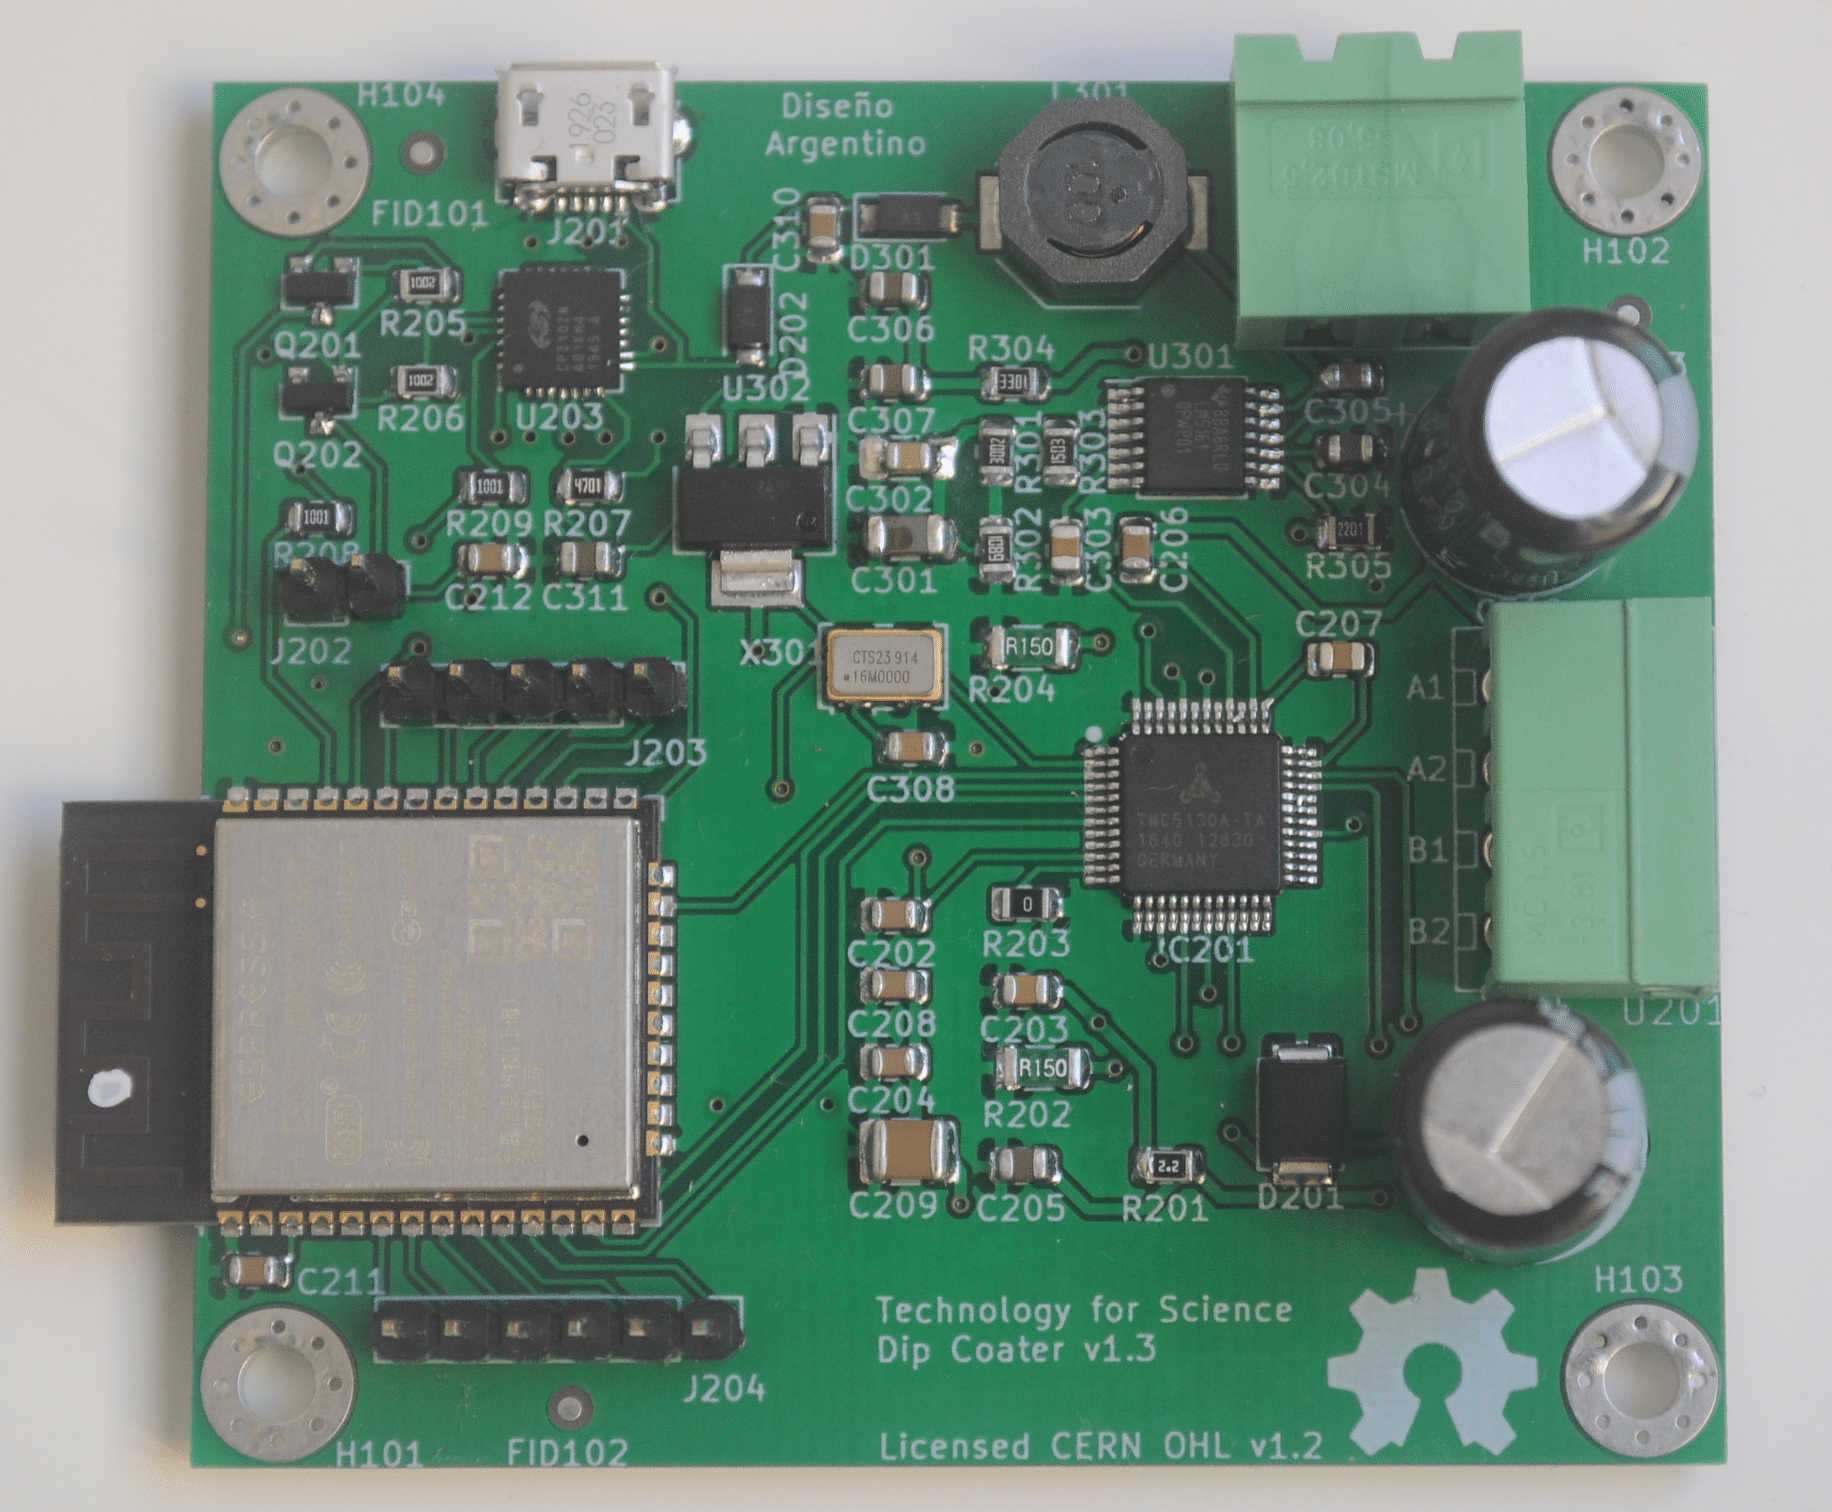
\includegraphics[width=.5\textwidth]{./Figures/dip_real_model.pdf}
	\caption{Placa fabricada MAYER SRL.}
	\label{fig:dip_real_model}
\end{figure}

  
%-----------------------------------
%	SUBSECTION 1
%-----------------------------------
\subsection{Diseño}
%-----------------------------------
%	SUBSECTION 2
%-----------------------------------
\subsection{Fabricación, pruebas y rediseño}


%----------------------------------------------------------------------------------------
%	SECTION 2
%----------------------------------------------------------------------------------------

\section{Software}

\subsection{Capas de abatracción}


%----------------------------------------------------------------------------------------
%	SECTION 3
%----------------------------------------------------------------------------------------

\section{Estructura mecánica}

\subsection{Diseño 3D}
\subsection{Fabricación de piezas a través de mecanizado CNC}


